%==============================================================================
% tento soubor pouzijte jako zaklad
% this file should be used as a base for the thesis
% Autoři / Authors: 2008 Michal Bidlo, 2018 Jaroslav Dytrych
% Kontakt pro dotazy a připomínky: dytrych@fit.vutbr.cz
% Contact for questions and comments: dytrych@fit.vutbr.cz
%==============================================================================
% kodovani: UTF-8 (zmena prikazem iconv, recode nebo cstocs)
% encoding: UTF-8 (you can change it by command iconv, recode or cstocs)
%------------------------------------------------------------------------------
% zpracování / processing: make, make pdf, make clean
%==============================================================================
% Soubory, které je nutné upravit: / Files which have to be edited:
%   projekt-20-literatura-bibliography.bib - literatura / bibliography
%   projekt-01-kapitoly-chapters.tex - obsah práce / the thesis content
%   projekt-30-prilohy-appendices.tex - přílohy / appendices
%==============================================================================
\documentclass[slovak,zadani,print]{fitthesis} % bez zadání - pro začátek práce, aby nebyl problém s překladem
%\documentclass[english]{fitthesis} % without assignment - for the work start to avoid compilation problem
%\documentclass[zadani]{fitthesis} % odevzdani do wisu a/nebo tisk s barevnými odkazy - odkazy jsou barevné
%\documentclass[english,zadani]{fitthesis} % for submission to the IS FIT and/or print with color links - links are color
%\documentclass[zadani,print]{fitthesis} % pro černobílý tisk - odkazy jsou černé
%\documentclass[english,zadani,print]{fitthesis} % for the black and white print - links are black
%\documentclass[zadani,cprint]{fitthesis} % pro barevný tisk - odkazy jsou černé, znak VUT barevný
%\documentclass[english,zadani,cprint]{fitthesis} % for the print - links are black, logo is color
% * Je-li práce psaná v anglickém jazyce, je zapotřebí u třídy použít 
%   parametr english následovně:
%   If thesis is written in english, it is necessary to use 
%   parameter english as follows:
%      \documentclass[english]{fitthesis}
% * Je-li práce psaná ve slovenském jazyce, je zapotřebí u třídy použít 
%   parametr slovak následovně:
%   If the work is written in the Slovak language, it is necessary 
%   to use parameter slovak as follows:
%      \documentclass[slovak]{fitthesis}
% * Je-li práce psaná v anglickém jazyce se slovenským abstraktem apod., 
%   je zapotřebí u třídy použít parametry english a enslovak následovně:
%   If the work is written in English with the Slovak abstract, etc., 
%   it is necessary to use parameters english and enslovak as follows:
%      \documentclass[english,enslovak]{fitthesis}

% Základní balíčky jsou dole v souboru šablony fitthesis.cls
% Basic packages are at the bottom of template file fitthesis.cls
% zde můžeme vložit vlastní balíčky / you can place own packages here

% Kompilace po částech (rychlejší, ale v náhledu nemusí být vše aktuální)
% Compilation piecewise (faster, but not all parts in preview will be up-to-date)
% \usepackage{subfiles}

% Nastavení cesty k obrázkům
% Setting of a path to the pictures
%\graphicspath{{obrazky-figures/}{./obrazky-figures/}}
%\graphicspath{{obrazky-figures/}{../obrazky-figures/}}

%---rm---------------
\renewcommand{\rmdefault}{lmr}%zavede Latin Modern Roman jako rm / set Latin Modern Roman as rm
%---sf---------------
\renewcommand{\sfdefault}{qhv}%zavede TeX Gyre Heros jako sf
%---tt------------
\renewcommand{\ttdefault}{lmtt}% zavede Latin Modern tt jako tt

% vypne funkci šablony, která automaticky nahrazuje uvozovky,
% aby nebyly prováděny nevhodné náhrady v popisech API apod.
% disables function of the template which replaces quotation marks
% to avoid unnecessary replacements in the API descriptions etc.
\csdoublequotesoff

% =======================================================================
% balíček "hyperref" vytváří klikací odkazy v pdf, pokud tedy použijeme pdflatex
% problém je, že balíček hyperref musí být uveden jako poslední, takže nemůže
% být v šabloně
% "hyperref" package create clickable links in pdf if you are using pdflatex.
% Problem is that this package have to be introduced as the last one so it 
% can not be placed in the template file.
\ifWis
\ifx\pdfoutput\undefined % nejedeme pod pdflatexem / we are not using pdflatex
\else
  \usepackage{color}
  \usepackage[unicode,colorlinks,hyperindex,plainpages=false,pdftex]{hyperref}
  \definecolor{hrcolor-ref}{RGB}{223,52,30}
  \definecolor{hrcolor-cite}{HTML}{2F8F00}
  \definecolor{hrcolor-urls}{HTML}{092EAB}
  \hypersetup{
	linkcolor=hrcolor-ref,
	citecolor=hrcolor-cite,
	filecolor=magenta,
	urlcolor=hrcolor-urls
  }
  \def\pdfBorderAttrs{/Border [0 0 0] }  % bez okrajů kolem odkazů / without margins around links
  \pdfcompresslevel=9
\fi
\else % pro tisk budou odkazy, na které se dá klikat, černé / for the print clickable links will be black
\ifx\pdfoutput\undefined % nejedeme pod pdflatexem / we are not using pdflatex
\else
  \usepackage{color}
  \usepackage[unicode,colorlinks,hyperindex,plainpages=false,pdftex,urlcolor=black,linkcolor=black,citecolor=black]{hyperref}
  \definecolor{links}{rgb}{0,0,0}
  \definecolor{anchors}{rgb}{0,0,0}
  \def\AnchorColor{anchors}
  \def\LinkColor{links}
  \def\pdfBorderAttrs{/Border [0 0 0] } % bez okrajů kolem odkazů / without margins around links
  \pdfcompresslevel=9
\fi
\fi
% Řešení problému, kdy klikací odkazy na obrázky vedou za obrázek
% This solves the problems with links which leads after the picture
\usepackage[all]{hypcap}

% Informace o práci/projektu / Information about the thesis
%---------------------------------------------------------------------------
\projectinfo{
  %Prace / Thesis
  project={BP},            %typ práce BP/SP/DP/DR  / thesis type (SP = term project)
  year={2019},             % rok odevzdání / year of submission
  date=\today,             % datum odevzdání / submission date
  %Nazev prace / thesis title
  title.cs={Zpracování výměnného formátu Informačního systému katastru nemovitostí},  % název práce v češtině či slovenštině (dle zadání) / thesis title in czech language (according to assignment)
  title.en={Processing of the Exchange Information Format of the Real Estate Cadastre Information System}, % název práce v angličtině / thesis title in english
  %title.length={14.5cm}, % nastavení délky bloku s titulkem pro úpravu zalomení řádku (lze definovat zde nebo níže) / setting the length of a block with a thesis title for adjusting a line break (can be defined here or below)
  %Autor / Author
  author.name={Martin},   % jméno autora / author name
  author.surname={Nizner},   % příjmení autora / author surname 
  %author.title.p={Bc.}, % titul před jménem (nepovinné) / title before the name (optional)
  %author.title.a={Ph.D.}, % titul za jménem (nepovinné) / title after the name (optional)
  %Ustav / Department
  department={UITS}, % doplňte příslušnou zkratku dle ústavu na zadání: UPSY/UIFS/UITS/UPGM / fill in appropriate abbreviation of the department according to assignment: UPSY/UIFS/UITS/UPGM
  % Školitel / supervisor
  supervisor.name={Radek},   % jméno školitele / supervisor name 
  supervisor.surname={Kočí},   % příjmení školitele / supervisor surname
  supervisor.title.p={prof. RNDr.},   %titul před jménem (nepovinné) / title before the name (optional)
  supervisor.title.a={Ing., Ph.D.},    %titul za jménem (nepovinné) / title after the name (optional)
  % Klíčová slova / keywords
  keywords.cs={Sem budou zapsána jednotlivá klíčová slova v českém (slovenském) jazyce, oddělená čárkami.}, % klíčová slova v českém či slovenském jazyce / keywords in czech or slovak language
  keywords.en={Sem budou zapsána jednotlivá klíčová slova v anglickém jazyce, oddělená čárkami.}, % klíčová slova v anglickém jazyce / keywords in english
  %keywords.en={Here, individual keywords separated by commas will be written in English.},
  % Abstrakt / Abstract
  abstract.cs={Do tohoto odstavce bude zapsán výtah (abstrakt) práce v českém (slovenském) jazyce.}, % abstrakt v českém či slovenském jazyce / abstract in czech or slovak language
  abstract.en={Do tohoto odstavce bude zapsán výtah (abstrakt) práce v anglickém jazyce.}, % abstrakt v anglickém jazyce / abstract in english
  %abstract.en={An abstract of the work in English will be written in this paragraph.},
  % Prohlášení (u anglicky psané práce anglicky, u slovensky psané práce slovensky) / Declaration (for thesis in english should be in english)
  declaration={Prohlašuji, že jsem tuto bakalářskou práci vypracoval samostatně pod vedením pana X...
Další informace mi poskytli...
Uvedl jsem všechny literární prameny a publikace, ze kterých jsem čerpal.},
  %declaration={Hereby I declare that this bachelor's thesis was prepared as an original author’s work under the supervision of Mr. X
% The supplementary information was provided by Mr. Y
% All the relevant information sources, which were used during preparation of this thesis, are properly cited and included in the list of references.},
  % Poděkování (nepovinné, nejlépe v jazyce práce) / Acknowledgement (optional, ideally in the language of the thesis)
  acknowledgment={V této sekci je možno uvést poděkování vedoucímu práce a těm, kteří poskytli odbornou pomoc
(externí zadavatel, konzultant, apod.).},
  %acknowledgment={Here it is possible to express thanks to the supervisor and to the people which provided professional help
%(external submitter, consultant, etc.).},
  % Rozšířený abstrakt (cca 3 normostrany) - lze definovat zde nebo níže / Extended abstract (approximately 3 standard pages) - can be defined here or below
  %extendedabstract={Do tohoto odstavce bude zapsán rozšířený výtah (abstrakt) práce v českém (slovenském) jazyce.},
  %faculty={FIT}, % FIT/FEKT/FSI/FA/FCH/FP/FAST/FAVU/USI/DEF
  faculty.cs={Fakulta informačních technologií}, % Fakulta v češtině - pro využití této položky výše zvolte fakultu DEF / Faculty in Czech - for use of this entry select DEF above
  faculty.en={Faculty of Information Technology}, % Fakulta v angličtině - pro využití této položky výše zvolte fakultu DEF / Faculty in English - for use of this entry select DEF above
  department.cs={ústav DEF}, % Ústav v češtině - pro využití této položky výše zvolte ústav DEF nebo jej zakomentujte / Department in Czech - for use of this entry select DEF above or comment it out
  department.en={DEF} % Ústav v angličtině - pro využití této položky výše zvolte ústav DEF nebo jej zakomentujte / Department in English - for use of this entry select DEF above or comment it out
}

% Rozšířený abstrakt (cca 3 normostrany) - lze definovat zde nebo výše / Extended abstract (approximately 3 standard pages) - can be defined here or above
%\extendedabstract{Do tohoto odstavce bude zapsán výtah (abstrakt) práce v českém (slovenském) jazyce.}

% nastavení délky bloku s titulkem pro úpravu zalomení řádku - lze definovat zde nebo výše / setting the length of a block with a thesis title for adjusting a line break - can be defined here or above
%\titlelength{14.5cm}


% řeší první/poslední řádek odstavce na předchozí/následující stránce
% solves first/last row of the paragraph on the previous/next page
\clubpenalty=10000
\widowpenalty=10000

% checklist
\newlist{checklist}{itemize}{1}
\setlist[checklist]{label=$\square$}

\begin{document}
  % Vysazeni titulnich stran / Typesetting of the title pages
  % ----------------------------------------------
  \maketitle
  % Obsah
  % ----------------------------------------------
  \setlength{\parskip}{0pt}

  {\hypersetup{hidelinks}\tableofcontents}
  
  % Seznam obrazku a tabulek (pokud prace obsahuje velke mnozstvi obrazku, tak se to hodi)
  % List of figures and list of tables (if the thesis contains a lot of pictures, it is good)
  \ifczech
    \renewcommand\listfigurename{Seznam obrázků}
  \fi
  \ifslovak
    \renewcommand\listfigurename{Zoznam obrázkov}
  \fi
  % \listoffigures
  
  \ifczech
    \renewcommand\listtablename{Seznam tabulek}
  \fi
  \ifslovak
    \renewcommand\listtablename{Zoznam tabuliek}
  \fi
  % \listoftables 

  \ifODSAZ
    \setlength{\parskip}{0.5\bigskipamount}
  \else
    \setlength{\parskip}{0pt}
  \fi

  % vynechani stranky v oboustrannem rezimu
  % Skip the page in the two-sided mode
  \iftwoside
    \cleardoublepage
  \fi

  % Text prace / Thesis text
  % ----------------------------------------------
  %===============================================================================
% Autoř: Martin Nizner 2019
\chapter{Úvod}

Táto bakalárska práca má za cieľ implementovať databázu, ktorá bude vhodná pre uloženie dát registru územnej identifikácie, adries a nehnuteľností. O obsluhu implementovanej databázy sa bude starať nástroj, ktorý je súčasťou výslednej bakalárskej práce. Tento nástroj bude užívateľom umožňovať naplnenie prázdnej implementovanej databázy všetkými potrebnými dátami z registru územnej identifikácie adries a nehnuteľností spolu s aktualizáciou tejto databázy. Navrhnutý nástroj spolu s databázou by mali uľahčiť rôznym informačným systémom a mapovým klientom prístup k dátam registru územnej identifikácie, adries a nehnuteľností tak, aby nemuseli sami získavať tieto dáta pomocou výmenného formátu, ale mohli si ich jednoducho načítať z navrhnutej databázy, ktorá bude  umiestnená na ich serveri.

Úvodná časť tejto práce sa venuje vysvetleniu riešenej problematiky od objasnenia pojmu RÚIAN až po získanie dát RÚIAN pomocou výmenného formátu (kapitola \ref{chapter1}). Jadro práce sa venuje návrhu databázového modelu (kapitola \ref{chapter2}) a implementácií nástroja pre spracovanie prvkov RÚIAN (kapitola \ref{chapter3}). Záver práce tvoria ukážkové dotazy nad implementovanou databázou (kapitola \ref{chapter4}) spolu s nápadmi na vylepšenie výsledného implementovaného nástroja, ktoré sú súčasťou záveru (kapitola \ref{chapter5}). 
\chapter {Vysvetlenie riešenej problematiky}
\label{chapter1}
Táto kapitola sa venuje vysvetleniu a objasneniu pojmov, ktoré sa týkajú riešenej problematiky. Kapitola v úvode popisuje register územných adries a nehnuteľností, ktorého dáta boli v tejto práci získané . V jadre kapitoly je podrobne popísaný výmenný formát RÚIAN, pomocou ktorého boli dáta RÚIAN získané.
\section{Register územných adries a nehnuteľností}
V polovici roku 2012 bol úspešne spustený systém základných registrov verejnej správy Českej Republiky. Jeden zo štyroch základných registrov je i register územnej identifikácie, adries a nehnuteľností. RÚIAN  je verejný zoznam, ktorý umožňuje užívateľom z verejnej, ale i komerčnej a akademickej sféry, diaľkový prístup cez internet \cite{Ruian}.
\label{struktura}
\section{Typy poskytovania údajov z RÚIAN}
Existuje niekoľko spôsob, ktoré umožňuju získanie údajov z RÚIAN. Všetky existujúce postupy sú uvedené v tejto podkapitole.
\subsection{Aplikácia verejného ďiaľkového prístupu}
Spôsob umožňuje nazerať a získavať dáta základného registru RÚIAN a tiež niektoré dáta editačného agendového informačného systému územnej identifikácie \cite{Isui} a informačného systému katastru nehnuteľností \cite{Iksn} pomocou aplikácie verejného diaľkového prístupu \cite{Vdpman}.
Pre prístup do aplikácie VDP\footnote{Verejný diaľkový prístup} nie je potrebná žiadna registrácia. Poskytované dáta z VDP sú zadarmo. Dáta poskytované prostredníctvom VDP nie sú referenčné, majú iba informačný charakter. Aplikácia VDP obsahuje nasledujúce funkcionality:
\begin{itemize}
\item vyhĺadanie aktuálnych i zrušených prvkov
\item zobrazenie detailných informácií k vybranému prvku
\item export jednotlivých prvkov RÚIAN vo formátoch PDF \cite{Pdf}, CSV \cite{Csv} a XML \cite{Xml}
\item zobrazenie RÚIAN prvkov na mape pomocou mapového klienta Marushka \cite{Marushka}
\item poskytnutie informácií o vybranom prvku k určitému dátumu v minulosti (iba od 1.7.2011 nakoľko VDP eviduje dáta až od tohto dátumu)
\item poskytnutie informácií o vlastníkovi pozemku alebo stavebného objektu (budovy) evidovaného v
katastri nehnuteľností pomocou presmerovania do aplikácie nazerania do katastru nehnuteľností \cite{Kn}.
\item overenie adresy vrátane vyhľadania adresy na základe neúplných údajov.
\item poskytnutie obsahu registru RÚIAN a ISÚI\footnote{Informačný systém územnej identifikácie} vo výmennom formáte RÚIAN, ktorý je načtrnutý v podkapitole \ref{vdpbegin}.
\end{itemize}
Ku všetkým funkcionalitám aplikácie VDP sa dá dostať pomocou úvodnej obrazovky aplikácie VDP\cite{Vdp}.

Keďže účelom projektu je získať dáta RÚIAN pomocou výmenného formátu RÚIAN, tak zo všetkých poskytovaných funkcionalít aplikácie VDP bola využitá iba funkcionalita slúžiaca pre poskytnutie obsahu registru RÚIAN vo výmennom formáte RÚIAN.
\subsection{Výmenný formát RÚIAN}
\label{vdpbegin}
Spôsob umožňuje získavať dáta z RÚIAN pomocou výmenného formátu RÚIAN.\cite{Vfr} Jedná sa o súbory vo formáte XML. Tieto súbory je možné sťahovať nasledujúcimi spôsobmi: 
\begin{itemize}
	\item{prostredníctvom aplikácie VDP (v rámci projektu bol zo všetkých možných spôsobo získania dát RÚIAN zvolený práve tento jeden spôsob)}
	\item{z internetových (URL) adries vrátených webovými službami službami informačného systému základných registrov \cite{Iszr} – dostupné iba orgánom
      štátnej správy a samosprávy (nie sú voľne prístupné širokej verejnosti)}
\end{itemize}
Analýze VFR\footnote{Výmenný formát RÚIAN} sa ďalej podrobne venuje kapitola \ref{VymennyFormat}
\subsection{Webové služby informačného systému základných registrov}
V rámci ISZR\footnote{Informačný systém základných registrov} fungujú štyri základné registre verejnej správy (\bf register osôb, register obyvateľov, RÚIAN, register práv a povinností\rm) \cite{Zr}.
Webové služby ISZR \footnote{Informačný systém základných registrov} slúžia pre komunikáciu a výmenu dát medzi registrovanými agendovými informačnými systémami\cite{Ais} so základnými registrami verejnej správy.
Služby sú publikované na eGON \cite{Egon} rozhraní systémov základných registrov.
\subsection{Súbory s hodnotami oddelenými čiarkami}
Súbory obsahujú dáta RÚIAN vo formáte CSV a sú generované raz za mesiac z úplneho VFR súboru. Pre každú obec existuje jeden samostatný CSV súbor\cite{Csv}. Tieto CSV súbory je možné získať pomocou apliácie nazerania do katastru nehnuteľností \cite{Kn}.

\section{Výmenný formát registru územných adries a nehnuteľností}
\label{VymennyFormat}
VFR predstavuje jednu z foriem získavania a poskytovania dát RUIÁN, pričom dáta RUIÁN sú pri tejto forme uložené vo forme súborov, ktoré obsahujú tieto dáta vo formáte VFR. Keďže účelom projektu je získanie dát RUIÁN práve pomocou VFR, tak je tejto kapitole v rámci teoretickej časti venovaná najvačšia pozornosť, keďže je nevyhnutné pochopiť do detailu tento formát dát, nakoľko má byť extrahovaný do databázy. Budú teda vysvetlené a objasnené všetky dôležité súčasti VFR od formátu súborov VFR až po formát URL \cite{Url} adries, na ktorých sú tieto VFR súbory uložené.
\section{Formát súborov VFR}
Súbory VFR sú väčšinou uložené a komprimované na URL adresách vo formáte {\bf gzip} (niekedy sa vyskytnú prípady, keď sú uložené vo formáte {\bf zip}). V týchto archívoch sa vždy nachádza presne jeden súbor vo formáte XML, v ktorom sa nachádza stromová štruktúra zložená z elementov, ktoré ohraničujú kolekciu údajov a elementov, ktoré ohraničujú hodnoty atribútov týchto kolekcií. Nakoľko táto stromová štruktúra obsahuje geografické prvky (napríklad. súradnice definičného bodu), je uložená vo formáte GML (konkrétne sa jedná o GML 3.2.1)\cite{Gml}. 
\section {Kolekcie údajov vo VFR}
Vo VFR existuje niekoľko rôznych kolekcií údajov. V tejto podkapitole budú bližšie predstavené tie kolekcie údajov, ktoré budú využité v navrhovanom databázovom modeli pre projekt. Pochopenie štruktúr týchto kolekcií údajov je nevyhnutné z pohľadu správneho návrhu jednotlivých databázových entít navrhovaného databázového modelu. \\ \\
{\bf Prvok VFR} je základnou kolekciou údajov vo VFR. Je to vlastne prvok RÚIAN zapísaný vo formáte GML a obsahuje vo svojej kolekcií všetky atribúty a kolekcie, ktoré spadajú pod daný prvok. Tieto kolekcie a atribúty slúžia pre popis územného celku, ktorý spadá pod daný prvok VFR (napríklad v prípade prvku VFR {\bf Obec} sú popísané všetky územné prvky, ktoré spadajú pod územný celok obec - ulice, časti obce a podobne). Každý prvok VFR teda popisuje určitý územný celok. V tabuľke \ref{prvkyVfr} sú uvedené všetky prvky VFR , ktoré boli vo forme tabuliek zahrnuté do navrhovaného databázového modelu (názvy prvkov VFR odpovedajú ich názvom v súboroch VFR). V tabuľke je u kažého prvku VFR uvedená tiež jeho nadradená kolekcia, ktorá v súboroch VFR obaĺuje všetky prvky VFR s daným názvom.
\begin{table}[H]
\centering
\caption{Prehľad prvkov VFR}
\label{prvkyVfr}
\resizebox{\textwidth}{100pt} {
\begin{tabular}{|c|c|c|c|c|}
\hline Názov prvku VFR & Popis & Nadradená kolekcia \\ \hline
Stat & popisuje územie štátu & Staty \\
RegionSoudrznosti & popisuje územie regiónu súdržnosti & RegionySoudrznosti\\
Vusc & popisuje územie vyššieho územne samosprávneho celku & Vusc\\
Kraj & popisuje územie kraja podľa zákona číslo č.36/1960 Sb. & Kraje \\
Okres & popisuje územie okresu & Okresy\\
Orp & popisuje správny obvod obce s rozšírenou pôsobnosťou & Orp\\
Pou & popisuje správny obvod obce s rozšírenou pôsobnosťou & Pou\\
Obec & popisuje územie obce & Obce\\
CastObce & popisuje územie časti obce & CastiObci\\
Mop & popisuje územie mestského obvodu v meste Praha & Mop \\
SpravniObvod & popisuje územie správneho obvodu v meste Praha & SpravniObvody\\
Momc & popisuje územie mestského obvodu a mestskej časti územne členeného statuárneho mesta & Momc\\
KatasralniUzemi & popisuje územie katastrálneho územia podľa  katastrálneho zákona č. 344/1992 Sb. & KatastralniUzemi\\
Ulice & popisuje územie ulice alebo iného verejného priestranstva & Ulice\\
Zsj & popisuje územie základnej sídelnej jednotky & Zsj\\ \hline
\end{tabular}
}
\end{table}
Všetky prvky VFR uvedené v tabuľke sú spravované v agendovom systéme ISÚI a sú ukladané vo svojej nadradenej kolekcií údajov (napríklad kolekcia údajov {\bf Obce} môže obsahovať jednu alebo niekoľko kolekcií údajov Obec). Prvok {\bf Stat} tvorí najväčšiu kolekciu údajov vo VFR, nakoľko obsahuje všetky podradené prvky katastrálnych území, obcí a pod. spolu z ich atribútami a kolekciami údajov. \\ \\
{\bf Cudzí kľúč} je kolekciou údajov, ktorá je súčasťou kolekcie prvku VFR a vždy obsahuje kód nadradeného prvku VFR. Príklad cudzieho kľúča v súbore VFR:
\begin{lstlisting}[language=XML]
<vf:Obec gml:id="OB.592251">
    <obi:Okres>
        <oki:Kod>3705</oki:Kod>
    </obi:Okres>
</vf:Obec>
 \end{lstlisting}
Tento príklad obsahuje cudzí kľúč kolekcie {\bf Okres} v nadradenej kolekcií {\bf Obec}. Pomocou tohto cudzieho kľuča je možné zistiť, do akého okresu daná obec patrí. \\ \\
{\bf MluvnickeCharakteristiky} - táto kolekcia údajov obsahuje skloňovacie pády (konkrétne druhý až siedmy pád okrem piateho pádu), ktoré sú využité u niektorých prvkov RÚIAN (napríklad prvok Obec). Každý skloňovací pád je znakový typ o dlžke 48 znakov. Príklad skloňovacích pádov v súbore VFR:
\begin{lstlisting}[language=XML]
<vf:Obec gml:id="OB.592251">
    <obi:MluvnickeCharakteristiky>
        <com:Pad2>Prahy</com:Pad2>
        <com:Pad3>Praze</com:Pad3>
        <com:Pad4>Prahu</com:Pad4>
        <com:Pad6>Praze</com:Pad6>
        <com:Pad7>Prahou</com:Pad7>
    </obi:MluvnickeCharakteristiky>
</vf:Obec>
\end{lstlisting}
Jedná sa o skloňovacie pády mesta Prahy. \\ \\
{\bf Geometria}
Táto kolekcia obsahuje informácie o geometrickom určení prvku VFR. Každý atribút kolekcie geometrie má v súboroch VFR prefix {\bf gml} a jedná sa o časť  XML súboru, ktorá je vo formáte GML. Kolekcia má viac typov, pričom v tejto práci boli využité iba dva typy tejto kolekcie : 
\begin{itemize}
    \item {\bf DefinicniBod} - tento typ kolekcie geometrie obsahuje {\bf x}-ovú a {\bf y}-ovú súradnicu definičného bodu prvku VFR a jednoznačne tak určuje presnú pozíciu daného prvku VFR na mape. Príklad kolekcie definičného bodu: 
    \begin{lstlisting}[language=XML]
<vf:Obec gml:id="OB.592251">
    <obi:Geometrie>
        <gml:MultiPoint gml:id="DOB.554782">
            <gml:pointMembers>
                <gml:Point gml:id="DOB.554782.1">
                    <gml:pos>-743100.00 -1043300.00</gml:pos>
                </gml:Point>
            </gml:pointMembers>
        </gml:MultiPoint>
    </obi:Geometrie>
</vf:Obec>
\end{lstlisting}
Súradnice definičného bodu sa nachádzajú v elemente {\bf gml:pos}, pričom v mapovom kliente (Marushka) sú použiteľné iba v prípade, keď sa odstráni úvodný znak pomlčky. Ostatné elementy sú z pohľadu obsahu elementu {\bf obi:Geometrie} pre využitie v mapových klientoch nezaujímavé.
\item{\bf GeneralizovaneHranice} - tento typ kolekcie geometrie obsahuje všetky súradnice polygónu, ktorý definuje územie daného prvku VFR. Príklad kolekcie generalizovaných hraníc:
\begin{lstlisting}[language=XML]
<obi:GeneralizovaneHranice3>
    <gml:MultiSurface gml:id="GOB.558567.3">
        <gml:surfaceMember>
            <gml:Polygon gml:id="GOB.558567.3.1">
                  <gml:exterior>
                    <gml:LinearRing>
                      <gml:posList>-833663.85 -1078072.78 -833596.36 
                      -1078192.40 -833506.20 -1078221.94 
                      -833534.02 -1078394.63 -833488.64 
                      </gml:posList>
                    </gml:LinearRing>
                </gml:exterior>
            </gml:Polygon>
        </gml:surfaceMember>
    </gml:MultiSurface>
</obi:GeneralizovaneHranice3>
\end{lstlisting}
Jednotlivé súradnice sa nachádzajú v elemente {\bf gml:posList} a sú oddelené medzerou. Pre ich využitie v mapovom kliente je potrebné rovnako ako v prípade kolekcie definičného bodu odstrániť úvodný znak pomlčky.
\end{itemize}
Okrem týchto typov kolekcie geometrie ešte existujú ďalšie dva typy tejto kolekcie ({\bf OriginalniHranice} a {\bf DefinicniCara}), ktoré však nebudú popísané z dôvodu ich nevyužitia v tejto práci. \\\\
Okrem vyššie uvedených kolekcií ešte VFR obsahuje ďalšie kolekcie údajov, ktoré však v tejto práci nie sú využité a preto nebudú bližšie špecifikované ({\bf NespavneUdaje}, {\bf BonitovaneDily}, {\bf ZpusobyOchranyPozemku + ZpusobyOchrany}, {\bf CislaDomovni}, {\bf DetailniTEA}).



\section {Základné dátové typy VFR}
Existuje niekoľko základných datových typov, ktoré sa vyskytujú v súboroch VFR a je potrebné sa s nimi zoznámiť z dôvodu správneho návrhu databázového modelu. Ku každému dátovému typu je v nasledujúcom zozname uvedený príklad atribútov, v ktorých sa daný dátový typ používa. Zoznam všetkých atríbutov, ktoré sa nachádzajú v súboroch VFR vrátane ich popisu a využitia v prvkoch VFR je uvedený v tabuľke \ref{atributes}.

Zoznam základných dátových typov VFR: 
\begin{itemize}
    \item {{\bf Integer} -  tento datový typ má celočíselný rozsah od -2147483648 do 2147483647. Datový typ sa najčastejšie vyskytuje v kóde prvku RÚIAN, keďže každý prvok RÚIAN musí obsahovať kód, ktorý je jedinečný a je jeho jednoznačným identifikátorom. Ďalej sa tento typ vyskytuje v rôznych číselných údajoch (napríklad počet bytov, počet podlaží u stavebného objektu).}
    \item{{\bf String} - jedná sa o znakový typ rôznej dĺžky. Najčastejšie sa tento typ vyskytuje v atribúte Názov prvku VFR, keďže každý prvok VFR musí obsahovať názov. Ďalej sa tento typ vyskytuje napríklad u prvkov obcí, kde dosahuje v niektorých prípadoch až štyritisíc znakov (atribúty VlajkaText a ZnakText).}
    \item{{\bf Boolean} - jedná sa o datový typ, ktorý môže nadobúdať iba jednu z dvoch hodnôt pravda / nepravda (true/false). Tento datový typ sa vyskytuje napríklad v atribúte NespravnyUdaj, ktorý určuje, či je daný VFR prvok správny, alebo či nie je jeho platnosť spochybnená.}
    \item{{\bf DateTime} - tento typ definuje výpis dátumu a času v tvare RRRR-MM-DDTHH:MM:SS (napríklad  2019-05-01T00:00:00). Typ sa najčastejšie vyskytuje v atribúte PlatiOd, ktorý u každého prvku VFR určuje začiatok platnosti (začiatok platnosti v RÚIAN).}
    \item{{\bf Long} - jedná sa o datový typ s celočíselným rozsahom väčším než Integer. U prvkov VFR sa teda používa v prípadoch, u ktorých je potrebné použiť vačšiu číselnú hodnotu, než umožňuje Integer (používa sa iba u atribútov IdTransakce a GlobalniIdNavrhuZmeny).}
    \item{{\bf base64Binary} - tento dátový typ sa používa pre vykreselnie obrázkov u prvkov VFR. Využiva sa teda v atribútoch VlajkaObrazek a ZnakObrazek (prvky VFR Obec a Stat)}.
\end{itemize}

\begin{table}[h]
\centering
\caption{Prehľad atribútov VFR a ich využitia v prvkoch VFR}
\label{atributes}
\resizebox{\textwidth}{210pt} {
\begin{tabular}{|c|c|c|c|c|}
\hline Atribút & Typ & Dĺžka & Popis & Prvky VFR \\ \hline
Kod & Integer & 2 až 9 & Kód prvku VFR & (*)\\
Nazev & String & 32 až 48 & Názov prvku vo VFR & (*) \\
Nespravny & Boolean & & Príznak nesprávnosti údaju & (*) \\
PlatiOd & DateTime & & Začiatok platnosti & (*) \\
PlatiDo & DateTime & & Koniec platnosti & (*) \\
IdTransakce & Long & 18 & identifikátor prvku VFR v databáze RÚIAN & (*) \\
GlobalniIdNavrhuZmeny & Long & 18 & identifkátor návrhu zmeny v ISÚI & (*) \\
Geometrie & Geometrie & & Geometrické údaje & (*) \\
NespravneUdaje &  NespravneUdaje & & Zoznam nesprávnych referenčných údajov & (*) \\
DatumVzniku & DateTime & & Skutočný dátum vzniku prvku & (*) - (Ulice) \\
MluvnickeCharakteristiky & MluvnickeCharakteristiky & & Druhý až siedmy skloňovací pád & Obec, CastObce, MOMC, KatastralniUzemi\\
NutsLau & String & 6 & Kód územného prvku VFR v NUTS / LAU & Stat, RegionSoudrznosti, VUSC, Okres, Obec \\
Stat & Cudzí kľuč & & Nadradený Stat & RegionSoudrznosti, Kraj \\
Vusc & Cudzí kľuč & & Nadradené Vúsc & Okres, Orp\\
SpravniObecKod & Integer & 6 & Kód nadradenej správnej obce & Orp, Pou\\
VlajkaText & String & 4000 & Text popisujúci vlajku obce & Obec, Momc\\
VlajkaObrazek & base64Binary & & Obrázok vlajky obce & Obec, Momc\\ 
ZnakText & String & 4000 & Text popisujúci znak obce & Obec, Momc\\
ZnakObrazek & base64Binary &  & Obrázok znaku obce & Obec, Momc\\
Orp & Cudzí kľúč & & Nadradená Orp & Pou\\
StatusKod & Integer & 2 & Status obce & Obec\\
Okres & Cudzí kľuč & & Nadradený Okres & Obec\\
Pou & Cudzí kľuč & & Nadradená Pou & Obec\\
CleneniSmRozsahKod & Integer & 2 & Rozsah členenia statuárneho mesta na
MOMC & Obec\\
CLeneniSmTypKod & Integer & 2 & Typ MOMC, na ktoré je statutárne mesto
rozčlenené & Obec\\
ExistujeDigitalniMapa & Boolean & & Príznak existencie digitálnej mapy & KatastralniUzemi\\
RizeniID & Long & 18 & indetifikátor riadenia v ISKN & KatastralniUzemi\\
Kraj & Cudzí kľuč & & Nadradený Kraj & Okres\\
SpravniMomcKod & Integer & 6 & Kód správneho MOMC & SpravniObvod\\
Vymera & Long & 18 & Vymera ZSJ v m2 & ZSJ\\
CharakterZsjKod & Integer & 4 & Prevažújúci spôsob využitia ZSJ & ZSJ\\ \hline

\end{tabular}
}
\end{table}

\section{Typy súborov VFR}
\label{kriteria}
Súbory VFR je možné na základe prvkov VFR rozdeliť na niekoľko rôznych typov podľa rôznych kritérií. V nasledujúcej podkapitole budú uvedené všetky typy súborov, ktoré VFR poskytuje pri vyhľadávaní pomocou aplikácie VDP. Na základe typov súborov, ktoré VFR poskytuje, je možné rozdeliť typy súborov VFR podľa štyroch základných kritérií, na ktoré bude táto podkapitola rozdelená : 
\begin{itemize}
    \item {obsah prvkov RÚIAN}
    \item{obsah atribútov}
    \item{časová platnosť}
     \item{pokrytie prvkov RÚIAN}
\end{itemize}
Na základe každého z vyššie uvedených kritérií sa dá určiť, o aký typ súboru VFR sa jedná. O súbore VFR sa teda dá vždy povedať, že sa skladá z viacerých typov (má typ určený na základe obsahu atribútov, typ určený na základe časovej platnosti a podobne). Každé kritérium obsahuje vždy dva typy súborov VFR. Všetky uvedené typy súborov sa dajú naklikať vo vyhľadávacom formulári VDP tak, aby sme získali požadovaný súbor VFR.
\subsection {Rozdelenie podľa obsahu prvkov RÚIAN}
Toto kritérium rozdelenia určuje, aké prvky RÚIAN sa v súbore VFR budú vyskytovať a obsahuje tieto typy súborov VFR:
\begin{itemize}
\item{{\bf Súbory typu štát až zsj} - Súbory zahŕňajú tieto prvky RÚIAN: Stat, RegionSoudrznosti, Vusc, Orp, Kraj, Okres, Obec, CastObce, Momc, Mop, SpravniObvod, KatastralniUzemi, ZSJ. Tento typ súborov sa oplatí využiť, keď potrebujeme prístupiť k základným územným celkom (nepotrebujeme analyzovať najnižšie územné celky).}
\item{{\bf Súbory typu obec a jej podradené prvky} - súbory zahŕňajú tieto prvky RÚIAN: Obec, CastObce, Momc, Mop, SpravniObvod, KatastralniUzemi, Zsj, Ulice, Parcela, StavebniObjekt, AdresniMisto. Tento typ súborov sa oplatí využiť, keď potrebujeme analyzovať najnižšie územné celky spadajúce pod obec, ktoré sa nenachádzajú v súboroch typu {\bf štát až zsj}. Pre každú obec existuje jeden samostatný súbor tohto typu.}
\end{itemize}

\subsection {Rozdelenie podľa obsahu atribútov}
Toto kritérium rozdelenia určuje, aké atribúty prvkov RÚIAN sa budú v súboroch VFR nachádzať a obsahuje tieto typy súborov VFR:
\begin{itemize}
\item{{\bf Súbory základnej dátovej sady} - súbory zahŕňajú iba textové atribúty prvkov RÚIAN a u atribútu {\bf Geometrie} iba  jeden typ - definičný bod. Tieto súbory sa oplatí použiť, keď nám postačia iba textové údaje o jednotlivých prvkoch RÚIAN a plánujeme lokalizovať jednotlivé prvky RÚIAN iba na základe ich definičného bodu.}
\item{{\bf Súbory kompletnej dátovej sady} - súbory môžu obsahovať okrem textových atribútov i binárne dáta (napríklad atribút {\bf VlajkaObrazek}) a okrem definičného bodu obsahujú jeden alebo viac ďalších typov atribútu {\bf Geometrie} (generalizované hranice a podobne). To, ktoré z týchto ďalších atribútov sa budú v súboroch VFR nachádzať sa určí pomocou vyhľadávacieho formulára VDP. Tento typ súborov sa oplatí využiť, keď plánujeme ukladať všetky údaje o jednotlivých RÚIAN prvkoch alebo plánujeme lokalizovať celé územie jednotlivých prvkov RÚIAN pomocou polygónov (napríklad pomocou generalizovaných hraníc )}. 
\end{itemize}

\subsection {Rozdelenie podľa časovej platnosti}
Na základe tohro rozdelenia možno prvky VFR rozdeliť na tieto typy súborov: 
\begin{itemize}
    \item {{\bf Platné súbory VFR} - jedná sa o prvky RÚIAN, ktoré nemajú určený atribút {\bf PlatiDo}, ktorý určuje koniec platnosti prvku RÚIAN. Vo vačšine prípadov sa využíva vždy tento typ súborov VFR.}
    \item{{\bf Historické súbory VFR} - tieto súbory VFR obsahujú prvky RÚIAN, ktoré už nie sú platné a boli vyradené z databázy platných prvkov RÚIAN. Súbory sa odlišujú od platných prvkov RÚIAN atribútom {\bf PlatiDo} určujúcim koniec ich platnosti}. 
\end{itemize}

\subsection{Rozdelenie podľa pokrytia prvkov RÚIAN}
Toto kritérium bolo zámerne uvedené pod vyššie uvedenými kritériami, nakoľko určuje, či sa v súboroch VFR budú nachádzať všetky prvky RÚIAN zvolené podľa vyššie uvedených kritérií alebo len niektoré. Kritérium je teda na najvyššej vrstve a obaľuje všetky ostatné kritéria. Na základe tohto kritéria možno rozdeliť prvky VFR na tieto typy súborov:
\begin{itemize}
    \item {{\bf Mesačné stavové súbory} - Obsahujú úplne všetky prvky RÚIAN zvolené podľa vyššie uvedených kritérií. Tieto typy súborov sa generujú vždy posledný deň v mesiaci a sú k dispozícii následujúci deň (prvý deň v nasledujúcom mesiaci). Každý mesiac je teda vygenerovaný vždy práve jeden súbor tohto typu. Tento typ súborov sa oplatí využiť v prípade, keď plánujeme exportovať všetky prvky RÚIAN spadajúce pod vyššie uvedené kritéria (napríklad ak vytvárame novú databázu súborov základnej dátovej sady).}
    \item{{\bf Denné zmenové súbory} - Tieto typy súborov môžu byť generované každý deň a majú rovnakú štruktúru ako mesačné stavové súbory. Generovanie v danom dni závisí na podmienke, či sú v danom dni nejaké nové zmeny oproti poslednému mesačnému stavovému súboru (nikdy sa nevytvára prázdny zmenový súbor).Nový mesačný stavový súbor (generovaný v posledný deň aktuálneho mesiaca) sa tvorí z posledného stavového súboru predchádzajúceho mesiaca doplneného o prvky RÚIAN, ktoré sa nachádzajú v denných zmenových súborov za aktuálny mesiac - tento typ súborov teda tvorí dôležitú súčasť pri tvorbe mesačných stavových súborov. Oproti mesačným stavovým súborom však má niekoľko nedostatkov: 
    \begin{itemize}
    \item{Pokiaľ dôjde k zmene akéhokoľvek atribútu prvku RÚIAN, tak do zmenového súboru sa dostane vždy celý tento prvok RÚIAN so všetkými jeho atribútmi (generujú sa teda aj nezmenené atribúty, ktoré generované byť nemuseli).}
    \item{Najmenšou časovou jednotkou, ktorá sa zaznamenáva u zmenových súborov je jeden deň. To má za
    následok to, že pokiaľ dôjde v jednom dni k viac zmenám (napríklad založenie prvku , zmena prvku, zrušenie prvku) u nejakého prvku RÚIAN, tak sa do zmenového súboru dostane iba posledná vykonaná zmena (napríklad ak v jednom dni prvok zrušíme aj založíme, tak sa vykoná iba jeho založenie - bude duplikovaný).}
    \item{Zmenové súbory sa negenerujú pre súbory typu obec a jej podradené prvky - nie je možné teda pravidelne aktualizovať tieto územné celky.}
    \end{itemize}
    }
    Tento typ súborov sa oplatí využiť, pokiaľ plánujeme aktualizovať už existujúcu databázu prvkov RÚIAN.
\end{itemize}

\section {Špeciálny VFR}
Všetky doteraz uvedené informácie o VFR sa týkali štandardného VFR. Od verzie VFR 1.8 však bol pridaný ku štandardnému VFR aj špeciálny VFR, ktorý sa delí na dva typy súborov:
\begin{itemize}
    \item {{\bf Súbory číselníkov} - Obsahujú dodatočné informácie k prvkom RÚIAN. Každý súbor číselníkov sa vždy skladá zo šiestich základných atribútov: kód, názov, skratka, popis, začiatok platnosti a koniec platnosti. Na súbory číselníkov odkazuju prvky štandardného VFR (napríklad prvok {\bf Zsj} a jeho atribút {\bf CharakterZsjKod}, ktorý odkazuje na kolekciu údajov {\bf CharakterZsj} v číselníku).}
    \item{{\bf Súbory volebných okrskov} - tento typ súborov obsahuje kolekciu údajov {\bf VolebneOkrsky}, ktorá obsahuje všetky prvky RÚIAN s názvom {\bf VolebniOkrsek}. Jedná sa o jedinú kolekciu prvkov RÚIAN, ktorá nie je súčasťou štandardného VFR. }
\end{itemize}
Pokiaľ uvažujeme rozdelenie typov súborov VFR na základe kritérií uvedených v podkapitole \ref{kriteria}, tak súbory špeciálneho VFR sa dá rozdeliť iba na základe rozdelenia podľa pokrytia prvkov RÚIAN, pričom súbory volebných okrskov obsahujú pri tomto kritériu iba typ mesačných stavových súborov (generujú sa iba raz mesačne - vždy tretí deň v mesiaci).
\section {Možnosti získania súborov VFR}
Aktuálne je možné súbory VFR získať pomocou dvoch spôsobov:
\begin{itemize}
    \item {Pomocou aplikácie VDP.}
    \item{Pomocou webových služieb ISZR.}
\end{itemize}
\subsection{Získanie súborov VFR z aplikácie verejného diaľkového prístupu}
Táto funkcionalita aplikácie VDP bola využitá z dôvodu získania potrebných URL, na ktorých sa nachádzajú súbory VFR s dátami RÚIAN pre navrhovanú aplikáciu, ktorá bude k týmto súborom pristupovať pomocou získaných URL. Do hlavného formuláru pre vyhľadávanie súborov štandartného VFR sa dostaneme po kliknutí na tlačítko {\bf Výměnný formát} nachádzajúce sa na úvodnej obrazovke aplikácie VDP.

Formulár pre vyhľadávanie súborov štandartného VFR je možné prepnúť na formulár pre vyhľadávanie súborov špeciálneho VFR a opačne pomocou navigačného menu {\bf Výmenný formát}, ktoré sa nachádza v ľavej časti stránky. Vo formulári pre vyhľadávanie súborov štandartného VFR je možné nastaviť tieto vyhľadávacie kritéria: 
\begin{itemize}
\item platnosť údajov ({\bf platné} alebo {\bf historické})
\item časový rozsah ({\bf úplna kópia} alebo {\bf zmenové súbory od určitého dátumu})
\item územné prvky ({\bf štát } alebo {\bf obec a podradené} - samostatné súbory obcí)
\item datová sada ({\bf základná} alebo {\bf kompletná})
\item výber z údajov ({\bf základné údaje}, {\bf generalizované hranice}, {\bf originálné hranice} a {\bf vlajky a znaky})
\item územné obmedzenie ({\bf celá ČR}, {\bf len konkrétny kraj}, {\bf len konkrétna obec s rozšírenou pôsobnosťou} a {\bf len konkrétná obec}
\end{itemize}
V prípade, že je za územný prvok zvolený štát  a súčasne je zvolená kompletná dátová sada, tak je potrebné vo výbere z údajov zvoliť aspoň jednu hodnotu okrem hodnoty základné údaje.
Formulár pre vyhľadávanie súborov špeciálneho VFR obsahuje iba položky časový rozsah a výber z údajov ({\bf číselníky} a {\bf volebné okresy}). Po kliknutí na tlačítko vyhľadať vo formulári sa pod formulárom zobrazí tabuľka s výsledkami, ktoré spĺňajú zadané vyhľadávacie kritéria. Z tohto zoznamu výsledkov je možné vyčítať URL adresy, ktoré sú potrebné pre navrhovanú aplikáciu(adresy sú uložené pod ikonou diskety v poslednom stĺpci tabuľky ({\bf uložit}). Aplikácia VDP bola teda z pohľadu projektu  využitá ako pomôcka pre získanie týchto URL adries. Podrobnému popisu týchto Url adries sa venuje podkapitola \ref{urlstruct}. V nasledujúcom obrázku je uvedený príklad formulára s vyplnenými vyhľadávacími kriteriami a tabuľkov výsledkov pre dané vyhľadávacie kritéria.
\begin{figure}[H]
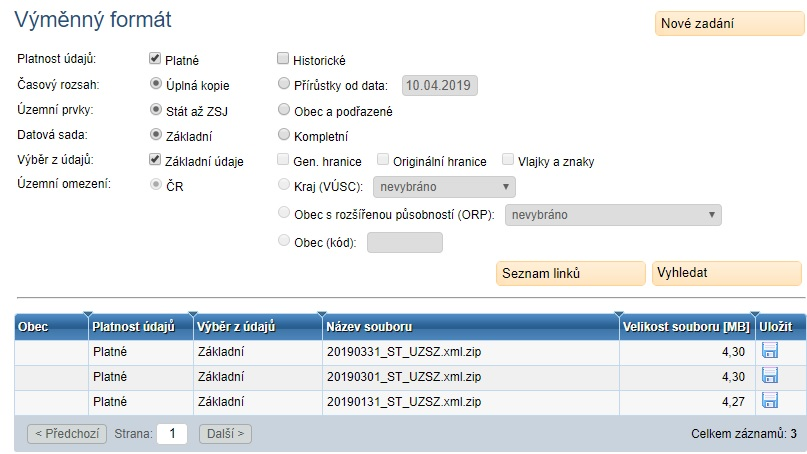
\includegraphics[width=\textwidth, height=8cm]{formularVDP}
\centering
\caption{Hlavný formulár pre vyhľadávanie súborov štadnartného VFR spolu s tabuľkou výsledkov.}
\end{figure}
\subsection {Získanie súborov VFR pomocou webových služieb registru územných adries a nehnuteľností}
Pri tomto spôsobe sú URL, na ktorých sa nachádzajú súbory VFR získané pomocou webových služieb RÚIAN. Tieto služby sú poskytované na eGON rozhraní ISZR. Aktuálne sú poskytované dva typy týchto webových služieb: 
\begin{itemize}
\item{{\bf E39 -  ruianSouboryZmen} - služba vracia zoznam súborov VFR zadaného typu, ktoré obsahujú zmenové súbory zvoleného prvku RÚIAN od zvoleného dátumu do súčasnosti. Dátum, od ktorého sú zmeny požadované, nesmie byť starši než tri mesiace. V prípade, že je zadaný typ súboru, ktorý nie je zmenovým typom, tak bude ako odpoveď vrátený prázdny XML súbor.
}
\item{{\bf E40 - ruianSouboryDat} - Služba vracia zoznam súborov VFR zadaného typu, ktoré obsahujú všetky údaje zvoleného prvku RÚIAN k poslednému dňu minulého mesiaca. V prípade, že je zadaný typ súboru, ktorý je zmenovým typom, tak bude ako odpoveď vrátený prázdny XML súbor.}
\end{itemize}
Tieto webové služby sú dostupné iba orgánom štátnej správy a samosprávy. Nakoľko tento spôsob získania súborov VFR nie je voľne prístupný širokej verejnosti, tak bol pre účely projektu jasne zvolený spôsob získania súborov VFR pomocou aplikácie VDP, ktorá je voľne prístupná širokej verejnosti.
\section{Štruktúra URL adries získaných pomocou aplikácie VDP}
\label{urlstruct}
Na základe experimentovania s aplikáciou VDP založenom na vyplňovaní rôznych kombinácií v hlavnom formulári pre vyhľadávanie súborov VFR bolo zistené, že kostru verejných URL adries, na ktorých sa nachádzajú súbory VFR, tvorí vždy tento základný tvar: vdp.cuzk.cz/{\bf a}/{\bf b}\_{\bf c}\_{\bf defg}.xml.{\bf i}, pričom význam jednotlivých zvýraznených neznámych je následujúci:
\begin{itemize}
\item{{\bf a} je u štandardného VFR typ súboru podľa kritéria časovej platnosti - {\bf soucasna} pre platné súbory a {\bf historicka} pre historické súbory. 
U špeciálneho VFR má táto neznáma v URL vždy pevnú hodnotu - {\bf specialni}}
\item{{\bf b} je formát dátumu v tvare {\bf YYYYMMDD} (deň, mesiac, rok)}
\item{{\bf c} je typ súboru podľa kritéria obsahu prvkov RÚIAN - {\bf ST} pre súbory typu štát  a {\bf OB\_kód-obce} pre súbory typu obec a podradené. U špeciálneho VFR má táto neznáma v URL vždy pevnú hodnotu {\bf ST}}
\item{{\bf d} je typ súboru podľa pokrytia prvkov RÚIAN - {\bf U} pre mesačné stavové súbory a {\bf Z} pre denné zmenové súbory.}
\item{\bf i} je typ archívu - gz alebo zip.
\end{itemize}
Neznáme {\bf e}, {\bf f} a {\bf g} majú tvoria vždy u súborov špeciálneho VFR nasledujúce hodnoty:
\begin{itemize}
    \item {{\bf CIS} pre súbory číselníkov}
    \item{{\bf VOH} pre súbory volebných okrskov.}
\end{itemize}
Naopak u súborov štandardného VFR má každá z týchto neznámych iný význam:
\begin{itemize}
    \item {{\bf e} je typ súboru podľa kritéria obsahu atribútov - {\bf Z} pre súbory základnej dátovej sady a {\bf K} pre súbory kompletnej dátovej sady.}
    \item{{\bf f} je typ súboru podľa časovej platnosti - {\bf S} pre platné súbory VFR a {\bf H} pre historické súbory VFR}
    \item {{\bf g} obsahuje dodatočné informácie k obsahu atribútov - {\bf Z} - iba atribúty základnej dátovej sady, {\bf G} - atribúty základnej dátovej sady spolu s geometriou generalizovaných hraníc, {\bf H} - základná dátová sada spolu s geometriou originálnych hraníc a {\bf O} - základná dátova sada spolu s obrázkami vlajok a znakov obcí.}
\end{itemize}
\subsection {Príklady URL adries súborov VFR}
V tejto podkapitole sú uvedené typické príklady URL adries na základe ich štruktúry popísanej v kapitole \ref{urlstruct} :
\begin{itemize}
    \item vdp.cuzk.cz/soucasna/20190301\_ST\_UZSZ.xml.gz - platný, mesačný stavový súbor základnej dátovej sady s prvkami RÚIAN štát .
    \item{vdp.cuzk.cz/soucasna/20190315\_ST\_ZKSG.xml.gz - platný, denný zmenový súbor kompletnej dátovej sady s geometriou generalizovaných hraníc a prvkami RÚIAN štát .}
    \item{vdp.cuzk.cz/soucasna/20190301\_OB\_500020\_ZKSO.xml.gz - platný, mesačný stavový súbor kompletnej dátovej sady s obrázkami vlajok a znakov obcí a prvkami RÚIAN obec a podradené.}
    \item{vdp.cuzk.cz/specialni/20190303\_ST\_UVOH.xml.gz - platný, mesačný stavový súbor kompletnej dátovej sady volebných okrskov.}
    \item{vdp.cuzk.cz/specialni/20190303\_ST\_UCIS.xml.gz - platný, mesačný stavový súbor kompletnej dátovej sady číselníkov} 
\end{itemize}
\chapter {Návrh databázového modelu}
\label{chapter2}
V tejto kapitole bude popísane, ktoré prvky RÚIAN boli zahrnuté do databázového modelu a budú podrobne vysvetlené jednotlivé časti databázového modelu.
\section {Zvolenie prvkov RÚIAN a ich atribútov pre export}
Na nasledujúcom obrázku sa nachádza zjednodušená schéma (stromová štruktúra) všetkých prvkov vedených v RÚIAN: 
\begin{figure}[H]
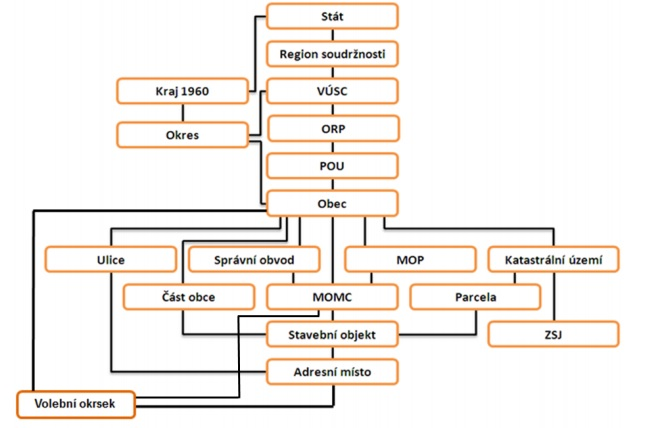
\includegraphics{schemaRuian}
\centering
\caption{Zjednodušená schéma prvkov RÚIAN \cite{Vdpman}.}
\label{schema}
\end{figure}
Keďže cieľom bakalárskej práce je exportovať predovšetkým súbory typu štát  základnej dátovej sady, tak medzi prvky RÚIAN určené pre návrh nebol zahrnutý prvok špeciálneho VFR (Volební okrsek) a niektoré prvky, ktoré sa nachádzajú v súboroch VFR typu obec a podradené (Parcela, Stavební objekt, Adresní místo). Všetky ostatné prvky RÚIAN, ktoré sú uvedené v obrázku \ref{schema}, boli do návrhu zahrnuté. Čo sa týka atribútov prvkov RÚIAN, tak do návrhu boli zahrnuté všetky atribúty uvedené v tabuľke \ref{atributes} okrem atribútov {\bf NespravneUdaje}(súčasťou návrhu aktuálne nie je kontrola správnosti údajov), {\bf GlobalniIdNavrhuZmeny}(cieľom navrhovanej aplikácie je práca s databázou RÚIAN a toto id sa týka databázy ISÚI) , {\bf RizeniID} (toto id sa týka databázy ISKN) a obrazových atribútov (ZnakObrazek, VlajkaObrazek), ktoré sú súčasťou kompletnej dátovej sady. Z typov geometrie bol do návrhu pre všetky prvky  RÚIAN zahrnutý základný typ geometrie okrem prvkov {\bf KatastralniUzemi} a {\bf Obec}, u ktorých boli do návrhu zahrnuté aj generalizované hranice. Originálne hranice neboli u žiadneho prvku RÚIAN do návrhu zahrnuté.
\section{Databázový model}
Navrhnutý databázový model tvorí aktuálne dvadsaťštyri entít a preto bol pre väčšiu prehľadnosť a ľahšie pochopenie rozdelený do niekoľko podkapitol, pričom každá podkapitola popisuje špecifickú časť databázového modelu. 
Primárny kľuč každej entity tvorí vždy hodnota atribútu {\bf Kod} a jeho veľkosť sa postupne navyšuje, nakoľko tvorí unikátny identifikátor v rámci celej databázy. Cudzie kľúče sú vždy uvedené v tvare {\bf id\_<nazov tabuľky>} a ich hodnotu tvorí hodnota primárneho kľúča tabuľky, na ktorú odkazujú. V prvých troch podkapitolách sú popísané časti modelu, ktoré nie sú súčasťou databázového model RÚIAN a pre zjednodušenie sú v nich uvedené len atribúty, ktoré sú pre tieto časti nevyhnutné. Posledné dve podkapitoly popisujú časti modelu, ktoré sú súčasťou databázového modelu RÚIAN a udávajú vzťahy medzi jednotlivými prvkami RÚIAN. 
\subsection {Základná geometria}
\label{basicGeometry}
Táto časť databázového modelu slúži pre uloženie definičných bodov všetkých prvkov RÚIAN a jej ER diagram je zobrazený na obrázku \ref{geometryEr}. Túto časť modelu tvorí vždy vzťah {\bf 1:1} - každý prvok RÚIAN má práve jeden jedinečný definičný bod v rámci celej databázy. Entita geometrie obsahuje okrem primárneho kľúču atribúty {\bf x\_axis} a {\bf y\_axis}, ktoré určujú definičný bod príslušného prvku RÚIAN. Táto časť databázového modelu bola zavedená z dôvodu redukcie počtu atribútov v jednotlivých entitách (v databázovom modeli RÚIAN každá entita obsahuje atribúty geometrie, ale v navrhovanom modeli bude vďaka tomuto riešeniu obsahovať atribúty geometrie iba jedna entita - {\bf geometry}).
\begin{figure}[H]
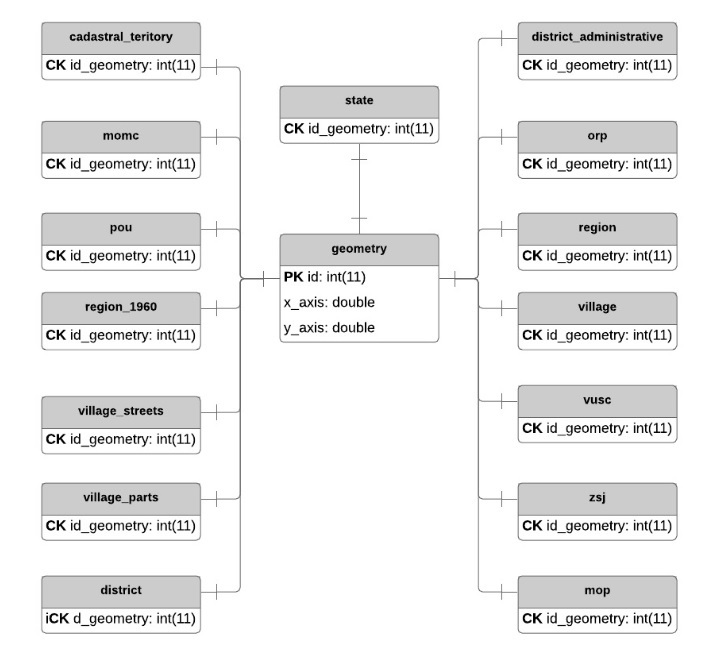
\includegraphics[height=14cm]{geometryEr}
\centering
\caption{Entita geometrie a jej vzťahy s entitami prvkov RÚIAN.}
\label{geometryEr}
\end{figure}
\subsection{Generalizované hranice}
ER diagram tejto časti databázového modelu je uvedený na obrázku \ref{coordinatesEr}. V tejto časti modelu sa nachádza vždy vzťah {\bf 1:N}, pričom na ľavej strane vzťahu sa nachádza prvok RÚIAN a na pravej strane vzťahu všetky súradnice jeho generalizovaných hraníc. V entite generalizovaných hraníc sa nachádza vždy jedna súradnica z kolekcie generalizovaných hraníc a cudzí kľúč, ktorý odkazuje na príslušný prvok RÚIAN. Táto časť databázového modelu tiež nie je súčasťou databázového modelu RÚIAN a bola zavedená z rovnakého dôvodu, ktorý je uvedený v podkapitole \ref{basicGeometry} (v tomto prípade každá entita obsahuje jeden atribút generalizovaných hraníc, v ktorom sú jednotlivé súradnice oddelené čiarkou). Oproti entite {\bf geometry} je tu však jedna nevýhoda - každý prvok RÚIAN, u ktorého sa ukladajú generalizované hranice, musí mať vlastnú entitu generalizovaných hraníc z dôvodu ukladania cudzieho kľúča v danej entite. Aktuálne sa ukladajú generalizované hranice pre entity {\bf village} a {\bf cadastral\_territory} - entity {\bf cadastral\_coordinates} a {\bf village\_coordinates} Ukladanie generalizovaných hraníc je do budúcnosti možné rozšíriť o ďalšie entity.
\begin{figure}[H]
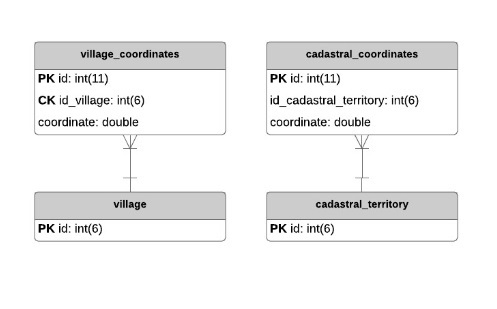
\includegraphics[height=7.5cm]{coordinatesEr}
\centering
\caption{Entity  generalizovaných hraníc spolu s entitami, ktoré ich využívajú.}
\label{coordinatesEr}
\end{figure}
\subsection {Skloňovacie pády}
Časť databázového modelu zabezpečuje uloženie skloňovacích pádov pre prvky RÚIAN, ktoré ich obsahujú. Návrh tejto časti modelu je uvedený na obrázku \ref{fallEr}. Vzťahy medzi jednotlivými entitami sú vždy typu {\bf 1:N}, pričom na ľavej strane vzťahu je prvok RÚIAN a na pravej starne vzťahu jeho skloňovacie pády. V entite skloňovacích pádov {\bf fall} sa nachádza atribút {\bf id\_main}, ktorý vždy odkazuje na úvodný druhý pád prvku RÚIAN a všetky entity prvku RÚIAN obsahujú cudzí kľúč {\bf id\_fall}, ktorý takisto odkazuje na druhý pád v entite {\bf fall}. Pomocou entity prvku RÚIAN je teda možné získať vždy iba druhý pád pre túto entitu. Následne je potrebné z entity {\bf fall} získať všetky ostatné pády pomocou atribútu {\bf id\_main}. Toto riešenie umožňuje mať iba jednu tabuľku skloňovacích pádov pre všetky prvky RÚIAN, ktoré obsahujú skloňovacie pády. Atribút {\bf no\_of\_fall} udáva číslo pádu podľa českého skloňovania \cite{czechFall}. Databáza RÚIAN ukladá skloňovacie pády vždy priamo v tabuľke prvku RÚIAN a preto až štyri tabuľky databázy RÚIAN obsahujú skloňovacie pády. V tomto návrhu obsahuje skloňovacie pády iba jedna tabuľka a sú v ňom zahrnuté všetky entity, ktoré skloňovacie pády využívajú. 
\begin{figure}[H]
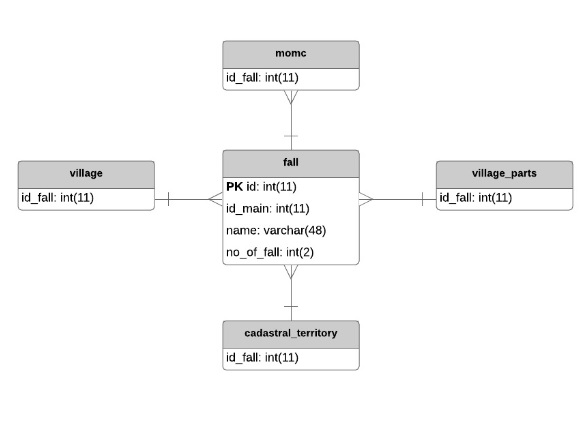
\includegraphics[height=10cm]{fallEr}
\centering
\caption{Návrh pre ukladanie skloňovacích pádov.}
\label{fallEr}
\end{figure}
\subsection {Súbory číselníkov}
Návrh tejto časti databázového modelu je uvedený na obrázku \ref{specialEr}.
Dva prvky RÚIAN, ktoré sú súčasťou návrhu databázového modelu ({\bf Obec} a {\bf Zsj}) obsahujú atribúty ({\bf CharakterZsjKod} a {\bf StatusKod}), ktoré odkazujú na súbory číselníkov (v súboroch číselníkov sa pod touto číselnou hodnotou nachádza názov charakteru Zsj respektíve typu obce). Z tohto dôvodu boli do návrhu zahrnuté entity {\bf village\_type} a {\bf zsj\_character}, ktoré uchovávajú potrebné názvy zo súborov číselníkov a nie je tak potrebné vyhľadávať tieto názvy v daných súboroch.
\begin{figure}[H]
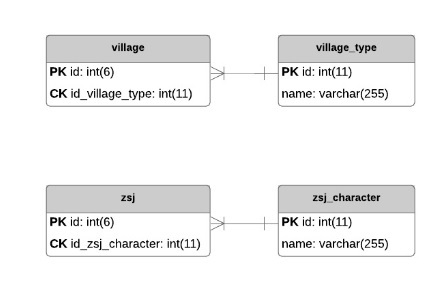
\includegraphics{specialEr}
\centering
\caption{Návrh pre ukladanie súborov číselníkov.}
\label{specialEr}
\end{figure}
\subsection{Prvá časť prvkov RÚIAN}
ER diagram tejto časti modelu je zobrazený na obrázku \ref{firstpartEr}. Táto časť databázového modelu je vo väčšine prípadov tvorená vzťahom {\bf 1:N}, kde na ľavej strane vzťahu je nadradená entita (nadradený väčší územný - napríklad {\bf state}) a na pravej strane vzťahu podradená entita (podradený menší územný celok - napríklad {\bf region\_1960}). Jedná sa o reťazové odkazovanie na väčšie nadradené územné celky  (obec  odkazuje na nadradenú entitu pou, následne pou odkazuje na nadradenú entitu orp, následne orp odkazuje na nadradenú entitu vusc, následne vusc odkazuje na nadradenú entitu region a na záver región odkazuje na nadradený štát). Okrem vzťahu 1:N sa v tejto časti ešte používa vzťah {\bf 1:0..1}, ktorý sa týka entít {\bf pou}, {\bf orp} a {\bf village}, kde entity {\bf orp} a {\bf pou} sú obce, ale neobsahujú všetky informácie, ktoré možno o obciach získať. Preto obsahujú cudzí kľúč odkazujúci na entitu {\bf village}, aby bolo možné o nich získať detailnejšie informácie.
\begin{figure}[H]
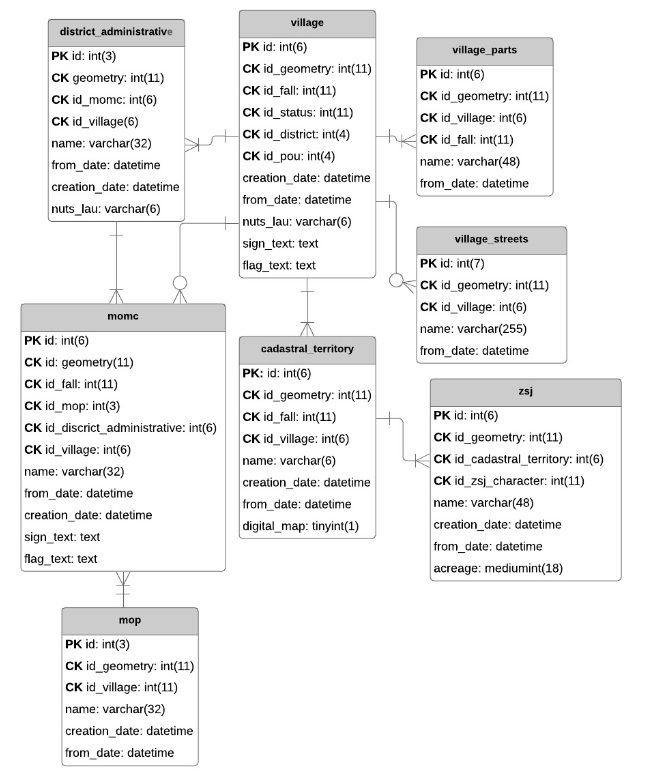
\includegraphics{firstPartEr}
\centering
\caption{Prvá časť prvkov RÚIAN}
\label{firstpartEr}
\end{figure}
\subsection{Druhá časť prvkov RÚIAN}
ER diagram tejto časti modelu je zobrazený na obrázku \ref{secondpartEr}
\begin{figure}[H]
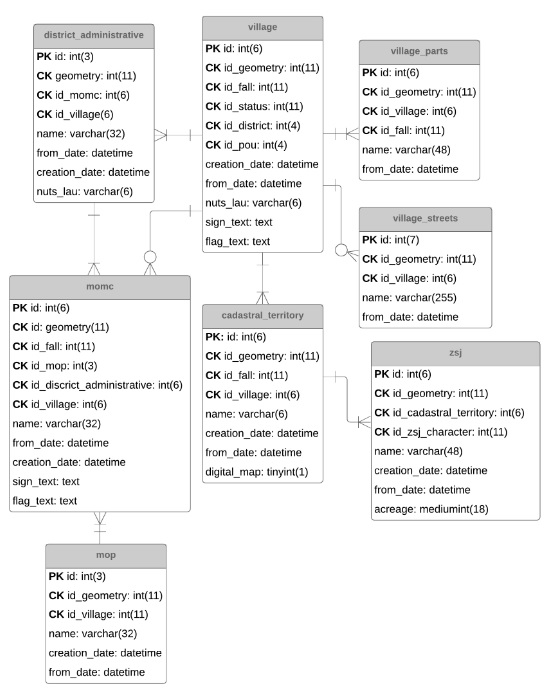
\includegraphics[height=17cm]{scondpartEr}
\centering
\caption{Druhá časť prvkov RÚIAN.}
\label{secondpartEr}
\end{figure}
Táto časť databázového modelu sa týka územného celku obce a jej podradených územných celkov. Vo väčšine prípadov sa v tejto časti používa medzi entitami vzťah {\bf 1:N}, kde na ľavej strane sa nachádza entita {\bf village} a na pravej strane jej podradený územný celok (niekedy je použitý vzťah {\bf 1:0..N} - napríklad vzťah medzi entitami {\bf village} a {\bf momc}, nakoľko niektoré obce vôbec nemajú mestský obvod).
\chapter {Implementácia nástroja pre spracovanie prvkov RÚIAN}
\label{chapter3}
Implementácia nástroja pre spracovanie prvkov VFR a ich uloženie do databázy je rozdelená na niekoľko dôležitých častí. Budú vysvetlené všetky súčasti implementovaného nástroja od použitých jazykov až po implementáciu databázy.
\section{Zvolenie implementačných nástrojov}
Implementovaný nástroj by mal jednorázovo vykonať potrebné operácie a následne ukončiť svoju činnosť. Z tohto dôvodu bolo rozhodnuté, že navrhovaný nástroj bude implementovaný v jazyku PHP.

Pre implementovanie databázy bol využitý z dôvodu bezproblémovej kompatibility na rôznych operačných systémoch a bezplatnej dostupnosti MySQL systém riadenia bázy dat.

Na základe týchto zvolených nástrojov je navrhovaný nástroj vlastne PHP skript pracujúci s MySQL databázou.
\section{Štruktúra skriptu}
Skript je rozdelený na niekoľko modelov a jednu pomocnú triedu. Každý z týchto modelov spolu s pomocnou triedou tvorí samostatný PHP súbor:
\begin{itemize}
    \item {\bf en.php} - pomocná trieda, ktorá obsahuje statické pole. Toto pole slúži pre preklad názvov prvkov a kolekcií súborov VFR do anglických názvov, ktoré sa využívajú v implementovanej databáze (kľúč tvorí anglický názov a hodnota tvorí český názov v súboroch VFR). Trieda sa nachádza v zložke languages.
    \item{Language.php} - model, ktorý obsahuje metódy pre prácu s pomocnou triedou {\bf en.php}.
    \item{{\bf XmlRuian.php} - model, ktorý slúži pre spracovanie súborov VFR - získa a roztriedi z nich dáta tak, aby boli pripravené pre vloženie do databázy}
    \item{{\bf RuianDatabase.php} - model, ktorý sa stará o operácie nad databázou - vykonáva vkladanie, odstraňovanie a aktualizovanie prvkov v implementovanej databáze.}
    \item{{\bf Ruian.php} - tento model tvorí jadro skriptu - začne vykonávať svoju činnost ihneď po spustení skriptu. Model sa stará sa o spracovanie argumentov príkazového riadku a riadenie činnosti ostatných modelov.}
\end{itemize}
\section{Spracovanie argumentov príkazového riadku VFR}
Po spustení skriptu prebehne v modeli {\bf Ruian.php} inicializácia ostatných modelov a kontrola argumentov príkazového riadku. Na základe argumentov príkazového riadku sa môže skript dostať do jedného z týchto dvoch stavov: \begin{itemize}
    \item {Pokiaľ je skript spustený bez parametrov, tak prebehne zmazanie všetkých záznamov aktuálnej databázy a budú sa spracovávať {\bf mesačné stavové súbory } VFR. Získane dáta zo súborov sa  uložia do prázdnej databázy.}
    \item{Pokiaľ je skript spustený s argumentom {\bf update}, tak prebehne spracovanie {\bf denných zmenových súborov}, ktorých spracované dáta sa následne použijú na vytvorenie nových alebo aktualizáciu existujúcich záznamov v databáze}.
\end{itemize} 

\subsection{Získanie URL adries a extrakcia súborov VFR z archívov}
Po spracovaní argumentov prikazového riadku predá ríadiaci model {\bf Ruian.php} riadenie skriptu modelu {\bf XmlRuian.php}. Tento model následne nastaví potrebné dátumové konštanty (prvý deň predchádzajúceho mesiaca pre mesačné stavové súbory a tretí deň predchádzajúceho mesiaca pre súbory číselníkov). Pri spracovaní denných zmenových súborov sa v cykle kontroluje  výskyt zmenových súborov od dátumu poslednej aktualizácie, ktorý je uložený v pomocnej tabuľke {\bf logs} až po dnešný dátum. Každá dátumová konštanta obsahuje niekoľko fáz kontroy, ktorá preverí existenciu URL adresy pre daný dátum:
\begin{itemize}
    \item {{\bf kontrola prípony archívu} - táto fáza sa vykonáva pri každej dátumove konštante. Kontrola najprv skontroluje, či existuje URL adresa s príponou súboru {\bf .gz}. V prípade neúspechu sa následne kontroluje existencia URL adresy s príponou {\bf .zip}}.
    \item{{\bf zmena dátumovej konštanty} - táto fáza sa vykoná iba v prípade neúspechu predošlej fázy a týka sa iba mesačných stavových súborov a súborov číseníkov. Fáza zmení v prípade neúspechu prvej fázy dátumovú konštantu pre mesačný stavový súbor na prvý deň aktuálneho mesiaca, nakoľko bolo občas narazené na takéto prípady vygenerovania súborov. V prípade súborov číselníkov sa dátumová konštanta upraví na tretí deň aktuálneho mesiaca. Po úprave dátumových konštant sa celá kontrola opakuje.}
\end{itemize}
Pokiaľ bola nájdená URL adresa pre zadanú dátumovu konštantu, tak prebehne uloženie archívu na disk. Následne sa vykoná extrakcia XML súboru z archívu (každý archív obsahuje práve jeden XML súbor). Subory XML sa ukladajú vždy do týchto zložiek v koreňovom adresári: \begin{itemize}
    \item {\bf files/vdp/base} pre mesačné stavové súbory kompletnej dátovej sady typu štát až ZSJ.
    \item{\bf files/vdp/villages} pre mesačné stavové súbory základnej dátovej sady typu obec a podradené.
    \item{\bf files/vdp/updates} pre denné zmenové súbory kompletnej dátovej sady
    \item{\bf files/vdp/dial} pre súbory číselníkov.
\end{itemize}
Samostatná zložka {\bf files} služi pre dočasné ukladanie stiahnutých archívov.
\section{Spracovanie extrahovaných XML súborov}
Z mesačného stavového súboru typu štát až zsj je možné získať všetky potrebné prvky VFR okrem prvku {\bf Ulice}, ktorý sa nachádza v mesačných stavových súboroch typu obec a podradené. Keďže pre každú obec existuje samostatný súbor s jej podradenými prvkami, tak je potrebné v prípade vytvárania novej databázy (denné zmenové súbory neobsahujú podradené prvky obce) vždy stiahnúť pre každú obec jej samostatný XML súbor (približne 6000 súborov), čo výrazne spomaľuje vykonávanie skriptu.

Model {\bf XmlRuian} obsahuje pre každý prvok VFR deklarované multidimenzionálne globálne pole, ktoré popisuje, čo všetko sa bude z daného prvku VFR extrahovať do databázy. Príklad takéhoto poľa pre prvok {\bf Stat}:
\begin{lstlisting}[language=PHP]
	private $state_collection = array('vf:Staty', 'vf:Stat', 
	array('sti:Kod', 'sti:Nazev', 'sti:PlatiOd', 'sti:NutsLau',
	'sti:DatumVzniku'), array());
\end{lstlisting}
Prvý index v poli obsahuje názov nadradenej kolekcie, ktorá obaľuje všetky prvky VFR s názvom, ktorý je uvedený v druhom indexe. Tretí index obsahuje pole názvov atribútov prvku {\bf Stat}, ktoré nie sú kolekciami. Posledný štvrtý index obsahuje pole názvov atribútov prvku {\bf Stat}, ktoré sú kolekciami (okrem kolekcie geometrie, ktorá sa spracúva samostatne a extrahuje sa povinne u každého prvku VFR). Tieto globálne polia je možné kedykoľvek upraviť a zmeniť tak dáta, ktoré budú zahrnuté do databázy.

Na začiatku spracovania XML súborov je deklarované pole {\bf all}, ktoré určuje, ktoré všetky prvky VFR sa budú extrahovať do databázy. Ak sa bude prvok VFR extrahovať do databázy, tak jeho multidimenzionálne globálne pole bude zahrnuté
do poľa {\bf all}. Aktuálne pole {\bf all} obsahuje všetky multidimenzionálne polia prvkov VFR, ktoré sú deklarované v modeli {\bf XmlRuian.php}.

Samotné spracovanie XML súborov prebieha pre každý samostatný XML súbor v cykle pomocou php rozširenia {\bf XmlReader}. Toto rozšírenie bolo vybraté z dôvodu rýchlejšieho spracovania XML súborov (narozdiel od niektorých iných nástrojov pre spracovanie XML tento nástroj neukladá celý obsah XML súboru do pamäte počítača, ale načíta potrebné dáta priamo z XML súboru, vďaka čomu prebieha spracovanie XML súboru rýchlejšie a je menej náročné pre pamäť počítača). Počas spracovania XML súboru sa získavané atribúty ukladajú do multidimenzionálného poľa {\bf ruianStructure}, ktorého kľúče prvej úrovne sú názvy tabuliek databázy (napríklad {\bf Stat}). Tieto kľúče obsahujú ďalšie pole s číselným indexovaním ([0], [1], [2]…), kde každý takýto číselný index predstavuje jeden záznam konkrétnej tabuľky a je tvorený ďalším poľom, ktorého kľúče sú názvy stĺpcov danej tabulky a obsahujú hodnotu priradenú danému stĺpcu tabuľky (napríklad {\bf[‘name’] => ‘Brno’}). Po kompletnom naplnení poľa {\bf RuianStructure} (pre denné zmenové súbory sa jedná o pole {\bf RuianStructuresFromUpdate}, ktoré obsahuje pre každý nájdený zmenový súbor samostatné pole {\bf RuianStructure}) sa ukončí činnosť modelu {\bf XmlRuian.php}, ktorý predá toto pole riadiacemu modelu {\bf Ruian.php}.
\section{Práca s databázou}
Prácu s databázou vykonáva databázový model {\bf RuianDatabase.php}. V tomto modeli sú definované konštanty ({\bf HOST}, {\bf DBNAME}, {\bf USER} a {\bf PASS}), ktoré slúžia pre úvodnú inicializáciu databázy a je možné ich kedykoľvek upraviť v závislosti na používanom databázovom serveri. Databázový model vykonáva prístup k databáze a dotazy nad ňou pomocou {\bf PDO} inštancie, ktorá je rozšíriteľnou súšasťou knižnice pre PHP. Spojenie s databázou sa vytvorí pri úvodnom vytvorení inštancie databázového modelu.

Ukladanie obsahu multidimenzionálneho poľa do databázy je rozdelené do niekoľkých fáz:
\begin{itemize}
    \item {{\bf príprava dát pre uloženie do databázy} - v tejto fáze riadiaci model {\bf Ruian.php} pre každý kĺúč prvej úrovne poľa {\bf RuianStructure} zavolá metódu {\bf prepareData}, ktorá hodnoty pod daným kĺúčom upraví pre konečné uloženie do databázy - uloži predčasne do databázy atribúty pod daným kľúčom, ktoré sú kolekciami prvkov a majú v databáze vytvorenú samostatnú tabuľku (generalizované hranice, skloňovacie pády)}. Upravené hodnoty sa nachádzajú v novom poli {\bf data\_to\_insert}. Kľúče tohto poľa sú preložené kľúče poľa {\bf RuianStructure}, v ktorom názvy kľučov odpovedajú názvom prvkov a ich atribútov v súboroch VFR. Preklad kľučov poľa {\bf RuianStructure} prebieha pomocou modelu {\bf Language.php}. Preložené kľuče poľa {\bf database\_to\_insert} odpovedaju názvom tabuliek a atribútov v implemetovanej databáze.
    \item {\bf uloženie dát do databázy} - v tejto fáze sa pre každý prvok poľa {\bf data\_to\_insert} zavolá v riadiacom modeli {\bf Ruian.php} metóda insert (pokiaľ záznam s daným prvkom už v databázi existuje, tak sa zavolá metóda {\bf update}) databázového modelu {\bf RuianDatabase.php}. Táto metóda vykoná uloženie tohto prvku do databázy. Jeden prvok poľa {\bf data\_to\_insert} predstavuje jeden záznam konkrétnej tabuľky a pole {\bf data\_to\_insert} predstavuje celkový obsah tejto tabuľky.
\end{itemize}
\chapter{Testovanie databázy}
\label{chapter4}
V tejto kapitole sa nachádzajú dotazy, ktoré boli využité pre otestovanie implementovanej relačnej databázy. Jedná sa o ukážkove dotazy, ktoré slúžia ako názorná ukážka práce s implementovanou relačnou databázou.Všetky dotazy sú uvedené v jazyku SQL a boli zádávané v nástroji phpMyAdmin. Pod každým dotazom je uvedený podrobnejší popis daného dotazu.
\\ \\
{\bf Prvý dotaz} - Počet obcí v Českej Republike.
\begin{lstlisting}[language=SQL]
SELECT COUNT(*) FROM village WHERE `id\_status` = '2'
\end{lstlisting}
Tento dotaz patrí medzi najjednoduchšie dotazy nad vytvorenou databázou. Dotaz pracuje iba s jednou tabuľkou (tabuľka {\bf village}) a jej jedným atribútom ({\bf id\_status}), ktorý je použitý vo {\bf where} klauzuly. Dotaz zobrazí počet záznamov v tabuľke {\bf village}, ktoré sú typu obce (jedná sa o jeden zo šesť typov). Pokiaľ chceme zistiť počet záznamov, ktoré sú iného typu tak zmeníme hodnotu atribútu {\bf id\_status} na hodnotu atribútu {\bf id} z tabuľky {\bf village\_type} tohto typu (napríklad hodnota {\bf id\_status} bude 4 pre zobrazenie počtu statuárnych miest v Českej Republike). \\ \\
{\bf Druhý dotaz} - Vypísanie súradníc polygónu, ktorý tvorí územie konkrétneho katastrálneho územia.
\begin{lstlisting}[language=SQL]
SELECT cadastral_coordinates.coordinate FROM cadastral_coordinates 
INNER 
JOIN cadastral_territory ON
cadastral_territory.id=cadastral_coordinates.id_cadastral_territory
WHERE cadastral_territory.name = 'Mesto Brno'
\end{lstlisting}
Oproti predchádzajúcemu dotazu je tento dotaz už o niečo zložitejší, nakoľko pracuje s dvoma tabuľkami a využíva klauzulu {\bf INNER JOIN}.
Tento konkrétny dotaz vypíše všetky súradnice katastrálneho územia mesta Brna. Tieto súradnice tvoria polygón, ktorý na mape zobrazuje územie tohto katastrálneho územia. Súradnice sa dajú využiť v rôznych mapových klientoch pre vykresľovanie súradníc konkrétneho katastrálneho územia v mape. Dotaz využíva dve tabuľky ({\bf cadastral\_territory} a {\bf cadastral\_coordinates}), ktoré sú medzi sebou prepojené na základe atribútov {\bf id\_cadastral\_territory} a {\bf id} pomocou klauzule {\bf INNER JOIN}. Zároveň dotaz obsahuje klauzulu {\bf WHERE}, ktorá udáva názov katastrálneho územia, pre ktoré chceme získať súradnice polygónu. \\ \\ \\ \\ \\ \\
{\bf Tretí dotaz} - Výpis {\bf x} -ovej a {\bf y}-ovej súradnice definičného bodu ľubovoľného prvku.
\begin{lstlisting}[language=SQL]
SELECT geometry.x_axis, geometry.y_axis FROM geometry 
INNER 
JOIN mop ON mop.id_geometry=geometry.id 
WHERE mop.name = 'Praha 2'
\end{lstlisting}
Tento typ dotazu možno aplikovať na tabuľku akéhokoľvek územného celku, nakoľko každá takáto tabuľka obsahuje atribút {\bf id\_geometry}, ktorý odkazuje na príslušný záznam v tabuľke {\bf geometry}. Tento konkrétny dotaz slúži pre vypísanie {\bf x}-ovej a {\bf y}-ovej súradnice definičného bodu mestského obvodu v Prahe s názvom Praha 2. Dotaz využíva tabuľku {\bf mop} a tabuľku {\bf geometry}, ktoré sú medzi sebou prepojené na základe atribútov {\bf id\_geometry} a {\bf id} pomocou klauzule {\bf INNER JOIN}. Klauzula {\bf where} určuje názov mestského obvodu v Prahe. Pokiaľ budeme chcieť vyhľadať súradnice definičného bodu v inej tabuľke na základe názvu územného celku tejto tabuľky, tak postačí zmeniť iba obsah klauzule {\bf FROM} (napríklad na {\bf 'village'} pre vyhľadávanie definičných bodov obcí). Tieto definičné body môžme rovnako ako v prípade súradníc polygónov využiť v rôznych mapových klientoch pre zobrazenie definičného bodu na mape. Súradnice je tiež možné použiť v {\bf Marushke}- klikneme na {\bf Hledat} v hornej časti pravej strany klienta a následne zvolíme možnosť {\bf Najdi souřadnice v S-JTSK}. Po zvolení tejto možnosti sa zobrazí formulár, do ktorého zadáme súradnice získané z databázového dotazu a formulár odošleme kliknutím na tlačítko {\bf Hledat}. Po odoslaní formuláru {\bf Marushka} zobrazí na mape definičný bod daného územného celku.
\\ \\
{\bf Štvrtý dotaz - výpis skloňovacích pádov konkrétnej obce}
\begin{lstlisting}[language=SQL]
SELECT fall.name, fall.id_fall_name FROM fall 
INNER JOIN village ON fall.id_main = village.id_fall 
WHERE village.name = 'Blatec'
\end{lstlisting}
Tento dotaz vypíše druhý až šiesty skloňovací pád konkrétnej obce. V tomto príklade sa jedná o obec Blatec. Dotaz využíva tabuľky {\bf fall} a {\bf village}, ktoré sú medzi sebou prepojené pomocou klauzule {\bf INNER JOIN} na základe atribútov {\bf id\_main} a {\bf id\_fall}. Klauzula {\bf WHERE} určuje názov obce, z ktorej chceme zobraziť skloňovacie pády. \\ \\
{\bf Piaty dotaz} - Výpis názvu a definičných bodov všetkých základných sídelných jednotiek typu priemyselný areál, ktoré sa nachádzajú v meste Brno
\begin{lstlisting}[language=SQL]
SELECT zsj.name, geometry.x_axis, geometry.y_axis FROM zsj 
INNER 
JOIN cadastral_territory ON zsj.id_cadastral_territory = cadastral_territory.id
INNER JOIN village ON cadastral_territory.id_village = village.id 
INNER JOIN geometry ON zsj.id_geometry = geometry.id 
WHERE village.name = 'Brno' AND zsj.id\_zsj\_character = '3';
\end{lstlisting}

Tento dotaz je oproti predchádzajúcim dotazom značne zložitejší a zobrazí názov všetkých základných sídelných jednotiek spolu s ich definičným bodom, ktoré sa nachádzajú v meste Brno. Dotaz pracuje s tabuľkami {\bf zsj}, {\bf cadastral\_territory}, {\bf village} a {\bf geometry}. Dotaz najprv prepojí tabuľky {\bf zsj} a {\bf cadastral\_territory} pomocou prvej {\bf INNER JOIN} klauzule na základe atribútov {\bf id\_cadastral\_territory} a {\bf id}. Druhá klauzula {\bf INNER JOIN} prepojí tabuľky {\bf cadastral\_territory} a {\bf village} na základe atribútov {\bf id\_village} a {\bf id}. Posledná klauzula {\bf INNER JOIN} získa definičné body základných sídelných jednotiek pomocou prepojenia tabuliek {\bf zsj} a {\bf geometry} na základe atribútov {\bf id\_geometry} a {\bf id}. Klauzula {\bf WHERE} určuje, že chceme získať základné sídelné jednotky z mesta Brna typu priemyselný areál. Pokiaľ by sme chceli zmeniť typ sídelnej jednotky, tak zmeníme hodnotu atribútu {\bf id\_zsj\_character} vo {\bf WHERE} klauzuli na hodnotu atribútu {\bf id} z tabuľky {\bf zsj\_character} tohto typu (napríklad hodnota {\bf id\_zsj\_character} bude 10 pre základné sídelné jednotky typu lesná plocha). Bolo by možné vyhľadávať aj podľa názvu typu základnej sídelnej jednotky rozšírením o ďalšiu klauzulu {\bf INNER JOIN}, ktorá by pracovala s tabuľkami {\bf zsj} a {\bf zsj\_character}. \\\\
{\bf Šiesty dotaz} - Výpis názvov miest Juhomoravského kraja
\begin{lstlisting}[language=SQL]
SELECT village.name FROM village 
INNER JOIN village_type ON village.id_status = village_type.id 
INNER JOIN district ON village.id_district = district.id 
INNER JOIN region_1960 ON district.id_region_1960 = region_1960.id 
WHERE region_1960.name = 'Jihomoravský' AND 
(village_type.name = 'Město' OR village_type.name = 'Statutární město' 
OR village_type.name = 'Hlavní město') ORDER BY village.name;
\end{lstlisting}
Jedná sa o dotaz, ktorý znie jednoducho, ale na základe väzieb medzi jednotlivými tabuľkami databázy je jeho štruktúra komplikovaná. Prvá klauzula {\bf INNER JOIN} spojí obec s jej typom pomocou prepojenia tabuliek {\bf village} a {\bf village\_type} na základe atribútov {\bf id\_status} a {\bf id}. Druhá klauzula {\bf INNER JOIN} prepojí obec s jej okresom prepojením tabuliek {\bf village} a {\bf district} na základe atribútov {\bf id\_district} a {\bf id}. Posledná klauzula {\bf INNER JOIN} prepojí okres s krajom prepojením tabuliek {\bf district} a {\bf region\_1960} na základe atribútov {\bf id\_region\_1960} a {\bf id}. Klauzula {\bf WHERE} určuje názov kraja ({\bf Jihomoravský}) a typ obce (keďže chceme získať všetky mestá je potrebné zahrnúť aj statuárne mestá a hlavné mesto). Na záver dotaz zoradí všetky mestá vzostupne podľa abecedy pomocou klauzule {\bf ORDER BY}.
\chapter{Záver}
\label{chapter5}
Na základe získaných poznatkov z naštudovania problematiky VFR bol vytvorený skript, ktorý umožňuje spracovávať súbory VFR a ukladať ich spracovaný obsah do naimplementovanej databázy. Skript aktuálne spracúva iba textové dáta bez obrazových dát vlajok a znakov.

Vznikol nástroj, ktorý umožňuje dostať údaje, ktoré sa nachádzajú v databáze RÚIAN pomocou VFR do naimplementovanej databázy, ktorá môže byť súčasťou akéhokoľvek webového rozhrania, informačného systému prípadne mapového klienta. Nástroj tak umožní spoločnostiam, ktoré ho budú využívať prístup k dátam RÚIAN pomocou naimplementovanej databázy (spoločnosti nebudú musieť využívať aplikáciu VDP a riešiť spracovanie VFR ale rovno pristúpia k dátam RÚIAN pomocou naimpelementovanej databázy).

V prílohe \ref{manual} je uvedený manuál slúžiaci  na spojazdnenie skriptu a databázy pri prvom spustení.

Na záver je uvedených ešte niekoľko nápadov na vylepšenie:
\begin{itemize}
\item{Výsledný skript by mohol byť rozšírený o ďalšie typy geometrie (napríklad definičné čiary ulíc), vďaka čomu by mohli rôzny mapový klienti zobrazovať na základe dát z databázy i územie ulíc.}

\item{Implementovaná databáza by mohla byť v budúcnosti rozšírená o ďalšie územné celky (hlavne územné celky zo súborov VFR typu {\bf Obec a podradené}, keďže z týchto súborov implementovaná databáza aktuálne uchováva iba prvok {\bf Ulice}.}

\item{Skript by mohol v budúcnosti kontrolovať pri spracovaní súborov VFR príznak {\bf NespravneUdaje} tak, aby sa do databázy dostali iba územné celky, ktoré sú platné k dátumu, v ktorom majú byť uložené do databázy.}
\item{Pre skript a databázu by mohlo byť do budúcna vytvorené webové rozhranie, s ktorým bude spúšťanie skriptu a zobrazenie údajov databázy príjemnejšie a jednoduchšie (dve tlačítka pre obsluhu skriptu - {\bf Create Database} a {\bf Update Database} a v prípade databázy výpis jednotlivých dát priamo vo webovom rozhraní bez nutnosti pristupovať k databáze napríklad pomocou nástroja phpMyAdmin).}
\end{itemize}






%===============================================================================

  
  % Kompilace po částech (viz výše, nutno odkomentovat)
  % Compilation piecewise (see above, it is necessary to uncomment it)
  %\subfile{projekt-01-uvod-introduction}
  % ...
  %\subfile{chapters/projekt-05-conclusion}


  % Pouzita literatura / Bibliography
  % ----------------------------------------------
\ifslovak
  \makeatletter
  \def\@openbib@code{\addcontentsline{toc}{chapter}{Literatúra}}
  \makeatother
  \bibliographystyle{bib-styles/slovakiso}
\else
  \ifczech
    \makeatletter
    \def\@openbib@code{\addcontentsline{toc}{chapter}{Literatura}}
    \makeatother
    \bibliographystyle{bib-styles/czechiso}
  \else 
    \makeatletter
    \def\@openbib@code{\addcontentsline{toc}{chapter}{Bibliography}}
    \makeatother
    \bibliographystyle{bib-styles/englishiso}
  %  \bibliographystyle{alpha}
  \fi
\fi
  \begin{flushleft}
  \bibliography{projekt-20-literatura-bibliography}
  \end{flushleft}

  % vynechani stranky v oboustrannem rezimu
  % Skip the page in the two-sided mode
  \iftwoside
    \cleardoublepage
  \fi

  % Prilohy / Appendices
  % ---------------------------------------------
  \appendix
\ifczech
  \renewcommand{\appendixpagename}{Přílohy}
  \renewcommand{\appendixtocname}{Přílohy}
  \renewcommand{\appendixname}{Příloha}
\fi
\ifslovak
  \renewcommand{\appendixpagename}{Prílohy}
  \renewcommand{\appendixtocname}{Prílohy}
  \renewcommand{\appendixname}{Príloha}
\fi
%  \appendixpage

% vynechani stranky v oboustrannem rezimu
% Skip the page in the two-sided mode
%\iftwoside
%  \cleardoublepage
%\fi
  
\ifslovak
%  \section*{Zoznam príloh}
%  \addcontentsline{toc}{section}{Zoznam príloh}
\else
  \ifczech
%    \section*{Seznam příloh}
%    \addcontentsline{toc}{section}{Seznam příloh}
  \else
%    \section*{List of Appendices}
%    \addcontentsline{toc}{section}{List of Appendices}
  \fi
\fi
  \startcontents[chapters]
  \setlength{\parskip}{0pt}
  % seznam příloh / list of appendices
  % \printcontents[chapters]{l}{0}{\setcounter{tocdepth}{2}}
  
  \ifODSAZ
    \setlength{\parskip}{0.5\bigskipamount}
  \else
    \setlength{\parskip}{0pt}
  \fi
  
  % vynechani stranky v oboustrannem rezimu
  \iftwoside
    \cleardoublepage
  \fi
  
  % Přílohy / Appendices
  
\chapter{Obsah priloženého CD}
\begin{itemize}
    \item {{\bf src}} - zdrojové súbory skriptu
    \item{{\bf tex}} - zdrojové súbory pre vytvorenie výsledného PDF dokumentu
    \item{{\bf php}} - súbory obsahujúce PHP verziu, ktorá bola použitá pre testovanie skriptu
    \item{{\bf sql}} - SQL súbory pre vytvorenie a testovanie databázy
\end{itemize}

\chapter{Manuál}
\label{manual}
V tejto prílohe je popísaný návod na vytvorenie databázy a spustenie skriptu.
\section {Vytvorenie databázy a jej prepojenie s PHP skriptom}
Vytvorenie databázy je popísane v nasledujúcich krokoch: 
\begin{itemize}
    \item {{\bf 1.}} Určíme si server, na ktorom budeme chcieť databázu založiť (napríklad lokálny MySql server pomocou nástroja Xampp - https://www.apachefriends.org/download.html
    \item {{\bf 2.}} Na danom serveri založíme novú databázu, do ktorej budeme chiceť ukladať dáta RÚIAN.
    \item{{\bf 3.} Nad založenou databázou spustíme sql {\bf sql/db.sql} (cesta z koreňového adresára skriptu)}
    \item{{\bf 4.} v súbore {\bf RuianDatabase.php}, ktorý je v koreňovom adresári skriptu vyplníme konštanty {\bf HOST}, {\bf DBNAME}, {\bf USER} a {\bf PASS} podľa konfigurácie serveru, na ktorom sme vytvorili databázu. Od tohto momentu je PHP skript prepojený s databázou.}
\end{itemize}
\section {Spustenie skriptu}
Skript je nutné spúšťať s verziou PHP 5 a vyššou. Daná verzia PHP musí mať nainštalované rozšírenie, ktoré umožňuje použiť triedu {\bf PDO}. Skript je možné spúštať pomocou jedného z dvoch spôsobov: 
\begin{itemize}
    \item {{\bf Spustenie skriptu bez parametrov} - slúži pre prvotné naplnenie databázy a používa sa pri prvom kontakte s databázou. Príklad spustenia v operačnom systéme Linux: 
    \begin{verbatim}
        php Ruian.php
    \end{verbatim}
    }
    \item{{\bf Spustenie skriptu s parametrom update} - služi pre aktualizáciu vyplnenej databázy a používa sa v prípade, keď chceme aktualizovať databázu o nové prvky v období od poslednej práce s databázou po súčasný dátum. Príklad spustenia v operačnom systéme Linux:
     \begin{verbatim}
        php -update Ruian.php
    \end{verbatim}}
\end{itemize}
Po naplnení databázy prvkami RÚIAN môžme databázu otestovať pomocou ukážkových sql súborov umiestnených v priečinku {\bf sql} koreňového adresára skriptu.




  
  % Kompilace po částech (viz výše, nutno odkomentovat)
  % Compilation piecewise (see above, it is necessary to uncomment it)
  %\subfile{projekt-30-prilohy-appendices}
  
\end{document}
